% COGENT: Cognitive Dimension-Aware Memory for Enhancing Code Agents
% AAAI 2027 Submission — English Version

\documentclass[letterpaper]{article} % DO NOT CHANGE THIS
\usepackage{aaai2027}  % DO NOT CHANGE THIS
\usepackage[hyphens]{url}  % DO NOT CHANGE THIS
\usepackage{graphicx} % DO NOT CHANGE THIS
\urlstyle{rm} % DO NOT CHANGE THIS
\def\UrlFont{\rm}  % DO NOT CHANGE THIS
\usepackage{natbib}  % DO NOT CHANGE THIS AND DO NOT ADD ANY OPTIONS TO IT
\usepackage{caption} % DO NOT CHANGE THIS AND DO NOT ADD ANY OPTIONS TO IT
\frenchspacing  % DO NOT CHANGE THIS

\usepackage{algorithm}
\usepackage{algorithmic}
\usepackage{newfloat}
\usepackage{listings}
\DeclareCaptionStyle{ruled}{labelfont=normalfont,labelsep=colon,strut=off} % DO NOT CHANGE THIS
\lstset{%
	basicstyle={\footnotesize\ttfamily},%
	numbers=left,numberstyle=\footnotesize,xleftmargin=2em,%
	aboveskip=0pt,belowskip=0pt,%
	showstringspaces=false,tabsize=2,breaklines=true}
\floatstyle{ruled}
\newfloat{listing}{tb}{lst}{}
\floatname{listing}{Listing}

\usepackage{amsmath}
\usepackage{amssymb}
\usepackage{booktabs}
\usepackage{multirow}
\usepackage{array}
\usepackage{xcolor}
\usepackage{tikz}
\usetikzlibrary{positioning, arrows.meta, matrix, fit, backgrounds, calc}

\pdfinfo{
/TemplateVersion (2027.1)
}

\setcounter{secnumdepth}{2} % Section and subsection numbering enabled for cross-references

\title{COGENT: Cognitive Dimension-Aware Memory for Enhancing Code Agents}

\author{
    Anonymous Authors\textsuperscript{\rm 1}
}
\affiliations{
    \textsuperscript{\rm 1}Anonymous Institution\\
    anonymous@example.com
}

\begin{document}

\maketitle

% ======================================================================
\begin{abstract}
LLM-based code agents solve programming tasks through tool-use trajectories, yet each problem is approached independently---operational knowledge from prior resolutions is discarded across episodes. While recent work on agent memory \cite{expel, reflexion, memgpt} and hierarchical memory organization \cite{g-memory, evolve-mem} has demonstrated the value of retaining past experience, existing systems organize memories either by temporal order, embedding proximity, or abstraction tier alone, neglecting the \emph{type of reasoning} encoded in each experience. We introduce \textsc{COGENT}, a memory framework that organizes code agent experience along a cognitive dimension axis (Causal, Contrastive, Strategic, Environment) crossed with an abstraction axis (Trajectory, Workflow, Summary, Insight), yielding a $4 \times 4$ structured memory lattice. For each incoming task, \textsc{COGENT} first elicits a cognitive profile diagnosing which reasoning dimensions the problem requires, then retrieves candidates via dual-channel similarity (task-level and cognition-level embeddings), re-ranks them through dimension-native LLM scoring where each memory is evaluated by its own cognitive category's criteria, and assembles a complementary triplet. Memories are injected entirely through the agent's system prompt with no model training. On 100 overlapping tasks from SWE-bench Verified (Django subset) using DeepSeek-V4-Flash, \textsc{COGENT} lifts the pass rate from 56.0\% (no-memory baseline) to 76.0\%, a 20 percentage point gain (22 tasks newly solved, 2 regressed). We further design a 20-condition ablation suite---spanning core pipeline ablations, cognitive dimension leave-one-out, abstraction tier leave-one-out, robustness checks, and multi-model validation---to isolate the marginal contribution of each system component, with all experiments implemented and currently executing.
\end{abstract}

\begin{links}
    % \link{Code}{https://github.com/example/cogent}
    % \link{Datasets}{https://example.com/datasets}
    % \link{Extended version}{https://arxiv.org/abs/XXXX.XXXXX}
\end{links}

% ======================================================================
\section{Introduction}

LLM-driven code agents---mini-swe-agent, SWE-Agent, OpenHands---routinely navigate repositories, inspect source files, execute shell commands, and synthesize patches for real-world software defects \cite{swe-agent, mini-swe-agent, openhands}. The canonical loop is familiar: an issue description arrives, the agent alternates between exploration and editing actions, and success is declared when the patch passes the accompanying test suite.

Yet a structural inefficiency persists. The diagnostic reasoning chain, the dead ends explored and abandoned, the causal links connecting symptoms to root causes---all this operational knowledge evaporates between episodes. An agent that spent thirty steps diagnosing a Django migration ordering violation will, when facing a structurally identical migration issue next, restart from zero: re-listing directories, re-reading configuration, re-mapping dependency graphs.

This observation has motivated a growing body of work on agent memory. Reflexion \cite{reflexion} maintains verbal self-reflections from failed attempts. ExpeL \cite{expel} systematically extracts cross-task insights by comparing successful vs.\ failed trajectories, managing an insight pool through ADD/EDIT/UPVOTE/DOWNVOTE operators. Hierarchical memory architectures---G-Memory's three-tier graph \cite{g-memory}, EVOLVE-MEM's self-adaptive hierarchy \cite{evolve-mem}, H-MEM's four-level index \cite{h-mem}---organize experiences at multiple abstraction granularities for efficient top-down retrieval. These advances collectively establish that retaining and reusing agent experience improves downstream task performance.

However, existing memory designs share a common organizing principle: memories are structured by \emph{what} they describe (which task, which repository, which abstraction tier) rather than \emph{what kind of reasoning} they encode. A memory about diagnosing a stale cache invalidation shares virtually no tokens with a query about a Django session timeout, yet both demand the same cognitive operation---trace the write path, check whether invalidation fires on the correct signal, verify the key namespace. Conversely, two memories that mention the same Django subsystem in near-identical language may encode entirely different reasoning types (one concerns template escaping, the other a database transaction boundary). Surface-form proximity is a noisy proxy for cognitive applicability.

\textsc{COGENT} departs from this paradigm by introducing a \emph{cognitive dimension axis} as a first-class organizing principle. Each memory entry is labeled not only by its abstraction tier but also by its cognitive facet---Causal (why did the error manifest? why does the fix work?), Contrastive (which approaches were tried and discarded? under what boundaries does the solution hold?), Strategic (what workflow design choices were made and why?), and Environment (what repository-specific conventions, toolchain quirks, and configuration traps were encountered?). Crossing these four cognitive facets with four abstraction tiers yields a $4 \times 4$ memory lattice where each of the 16 positions houses a distinct category of operational knowledge.

The retrieval side mirrors this structure. When a new task arrives, \textsc{COGENT} first elicits a \emph{cognitive profile} characterizing which reasoning dimensions the problem demands. This profile drives two parallel embedding channels: a task-level channel matching concrete semantics (file names, error messages, function signatures) and a cognition-level channel matching abstract reasoning patterns (causal chain topology, anti-pattern signatures). Candidates are then \emph{dimension-natively re-ranked}: each memory is evaluated by the scoring criterion appropriate to its own cognitive facet (causal memories by causal-chain isomorphism, environment memories by repository-region overlap), with dimensions the profile deems irrelevant receiving a penalty. Finally, a greedy selector assembles the final memory set, penalizing near-duplicate pairs and rewarding complementary facet combinations.

\textsc{COGENT} operates purely through prompt injection---all selected memories are concatenated into the agent's system message before task execution. This black-box design requires no parameter updates, no architectural modifications, and no coupling to any specific LLM, making it immediately deployable with any API-accessible code agent.

Our contributions are:

\begin{enumerate}
    \item[(C1)] A cognitive facet taxonomy for code agent memory---Causal, Contrastive, Strategic, Environment---that categorizes experiences by reasoning type rather than surface content alone, and a $4 \times 4$ memory lattice crossing these facets with abstraction tiers to create a two-dimensional organization distinct from purely hierarchical or flat memory stores.
    \item[(C2)] A retrieval protocol incorporating cognitive profile elicitation (diagnosing a query's reasoning needs before retrieval), dual-channel similarity matching (task-level and cognition-level embeddings with weighted fusion), and dimension-native re-ranking (scoring each candidate by its own cognitive category's criteria).
    \item[(C3)] An incremental sequential memory accumulation paradigm where the pool expands round-by-round, each solved task contributing its extracted lattice to the shared store, enabling measurement of marginal per-task memory contribution under a realistic continual-deployment regimen.
    \item[(C4)] A comprehensive 20-condition ablation design covering core pipeline ablations, cognitive dimension leave-one-out, abstraction tier leave-one-out, retrieval robustness checks, and multi-model validation---all implemented and currently executing.
    \item[(C5)] Empirical demonstration on 100 SWE-bench Verified Django tasks: \textsc{COGENT} achieves a 76.0\% pass rate against a 56.0\% no-memory baseline, a 20 percentage point net gain (22 tasks improved, 2 regressed).
\end{enumerate}

% ======================================================================
\section{Related Work}

\subsection{Experience Extraction from Agent Trajectories}

The idea of distilling reusable knowledge from agent execution traces has been explored extensively. Reflexion \cite{reflexion} pioneered verbal self-reflection: after a failed episode, the agent analyzes its own trajectory and produces a natural-language diagnosis, which is prepended to the prompt on the next attempt. ExpeL \cite{expel} generalized this to cross-task insight extraction, using an LLM to compare successful vs.\ failed trajectories on the same task and to identify common success patterns across different tasks, maintaining an evolving insight pool with explicit add, edit, upvote, and downvote operations. CTIM-Rover \cite{ctim-rover} subsequently attempted to apply ExpeL's experiential learning to software engineering agents but found that repository-level cross-task memory introduced noise that biased agents toward irrelevant tokens, highlighting the challenge of \emph{selective} retrieval that our dimension-aware approach addresses. DoT-Bank \cite{dot-bank} and Agent Workflow Memory \cite{awm} further advanced trajectory-to-memory distillation with diverse reflection strategies and workflow extraction.

\textsc{COGENT} builds on this lineage---we also extract structured memories from completed trajectories---but differs fundamentally in the \emph{organizing schema}. Where ExpeL stores insights as an unstructured natural-language pool managed by voting, and Reflexion maintains per-task verbal reflections, \textsc{COGENT} imposes a two-dimensional cognitive structure (facet $\times$ tier) that enables retrieval matched to the cognitive demands of the query rather than generic similarity.

\subsection{Hierarchical Memory Architectures}

Multi-tier memory organization has recently attracted substantial attention. G-Memory \cite{g-memory} structures multi-agent interaction traces as a three-level graph (Insight Graph $\rightarrow$ Query Graph $\rightarrow$ Interaction Graph) with bidirectional top-down/bottom-up traversal. EVOLVE-MEM \cite{evolve-mem} implements a self-adaptive hierarchy with a Dynamic Memory Network, a Hierarchical Memory Manager, and a Self-Improvement Engine that triggers reorganization based on retrieval quality metrics. H-MEM \cite{h-mem} proposes a four-level positional index (Domain $\rightarrow$ Category $\rightarrow$ Memory Trace $\rightarrow$ Episode) for O(1) routing efficiency. Agent-Memo uses filesystem-inspired tiered loading with abstract, overview, and full-content levels. These systems demonstrate the value of organizing memory at multiple granularities, and our abstraction tier axis (Trajectory $\rightarrow$ Workflow $\rightarrow$ Summary $\rightarrow$ Insight) shares this motivation. Where \textsc{COGENT} diverges is in adding a second, orthogonal axis: the cognitive facet. Rather than organizing solely by abstraction granularity, we cross abstraction tiers with reasoning types, creating a lattice where each coordinate represents a distinct \emph{kind} of useful knowledge.

\subsection{Retrieval with Redundancy Control and Complementarity}

Several recent systems address the problem of selecting complementary, non-redundant information from a candidate pool. Context-Picker \cite{context-picker} uses a two-stage GRPO-based reinforcement learning schedule where the second stage tightens redundancy margins to prune distractors, mining minimal sufficient evidence sets via leave-one-out pruning. MEM1 \cite{mem1} learns to synergize memory consolidation and reasoning through end-to-end RL, strategically discarding redundant information. MemFly \cite{memfly} formalizes memory selection as an Online Information Bottleneck problem, minimizing compression entropy while maximizing relevance. Our synergy-aware greedy selection---with explicit pairwise redundancy penalties (same tier, same facet, high cosine similarity) and complementarity bonuses (same source task, different cognitive facets)---operates in the same problem space. Relative to these learned approaches, our rule-based pairwise adjustments are simpler and require no training, but share the core insight that memory selection should optimize joint coverage rather than independent per-item scores.

\subsection{Cognitive Science Foundations}

The design of \textsc{COGENT}'s cognitive facet taxonomy is informed by well-established findings in human memory research. Tulving's episodic-semantic distinction \cite{tulving-episodic} separates memory for specific events from memory for general knowledge, motivating our abstraction axis. Schank's dynamic memory theory \cite{schank-dynamic} argued that remindings across superficially dissimilar situations are mediated by shared thematic structures (MOPs, scripts), which directly motivates our claim that cognitive facet alignment can surface relevant memories that lexical search would miss. The encoding specificity principle \cite{tulving-encoding}---retrieval is most effective when encoding and retrieval contexts overlap---provides grounding for our cognitive profile extraction step. Recent LLM agent memory systems including DCPM \cite{dcpm} and CDMem \cite{cdmem} have also drawn on cognitive science, though their organizing principles (dual-process theory, context-dependent indexing) differ from our facet-based taxonomy.

% ======================================================================
\section{Methodology}

We describe \textsc{COGENT} along three dimensions: the cognitive facet taxonomy that organizes memory by reasoning type (Section~\ref{sec:taxonomy}), the retrieval pipeline that selects memories for each query (Section~\ref{sec:retrieval}), and the sequential memory accumulation protocol (Section~\ref{sec:pool}). Memory construction from completed trajectories follows established extraction practices \cite{expel, reflexion}: raw trajectories are first summarized into structured records, then four LLM calls---one per abstraction tier---each jointly extract entries for all four cognitive facets (16 cells from 4 calls rather than 16). We omit detailed description of this standard extraction procedure and focus on what is distinctive: the cognitive facet taxonomy and the retrieval mechanisms built upon it.

% ----------------------------------------------------------------------
\subsection{Cognitive Facet Taxonomy}
\label{sec:taxonomy}

The central idea in \textsc{COGENT} is that memories of past debugging episodes should be organized by the \emph{type of reasoning} they encode, not merely by what they describe. We define four cognitive facets, each capturing a distinct mode of thought that code agents engage in during debugging:

\begin{itemize}
    \item \textbf{Causal}: Diagnostic reasoning about cause and effect. A causal memory traces the logical pathway from trigger to resolution---identifying what category of error occurred, what underlying mechanism produced it, and why the chosen intervention restores correct behavior. These memories answer \emph{why} questions.
    \item \textbf{Contrastive}: Comparative knowledge that distinguishes effective from ineffective approaches. A contrastive memory records approaches that were tried and abandoned (and the reason each failed), approaches that succeeded (and the discriminative feature that made the difference), and the boundary conditions under which a successful strategy remains valid. These memories answer \emph{what distinguishes} questions.
    \item \textbf{Strategic}: Knowledge about process and planning. A strategic memory captures decision criteria for choosing among alternative approaches, justifications for workflow design choices, risk-assessment heuristics, and guidelines for structuring the debugging process itself---not what was done, but why it was done that way. These memories answer \emph{how to approach} questions.
    \item \textbf{Environment}: Repository-specific and toolchain-specific operational knowledge. An environment memory records directory layout conventions, dependency graph structure, test framework invocation patterns, common configuration pitfalls (such as migration ordering constraints or fixture loading semantics), and tool invocation idioms. These memories answer \emph{where and how} questions within a particular codebase.
\end{itemize}

The choice of these four facets is grounded in an analysis of code agent failure modes on SWE-bench. Inspection of failed trajectories reveals that agent errors cluster into four categories: (i) misidentifying the causal mechanism linking symptom to root cause (Causal), (ii) persisting with a superficially plausible but ultimately incorrect fix strategy (Contrastive), (iii) following an inefficient or misguided exploration order (Strategic), and (iv) failing to discover repository-specific conventions or toolchain behavior (Environment). The four facets directly target these observed failure categories.

Each memory is also assigned an abstraction tier, following the hierarchical organization common in prior work \cite{g-memory, evolve-mem, h-mem}---ranging from concrete operational traces (Trajectory) through procedural patterns (Workflow) and diagnostic synopses (Summary) to cross-task methodological principles (Insight). Crossing the four cognitive facets with these four abstraction tiers yields a $4 \times 4$ lattice where each of the sixteen positions captures a distinct category of operational knowledge: a causal insight differs from a causal trajectory trace, an environment workflow differs from an environment summary, and so on.

\subsubsection{Memory Entry Structure}
\label{sec:entry}

Each entry in the memory store carries three components, each serving a distinct role in downstream retrieval.

\textbf{Cognitive abstract.} A short, decontextualized summary of the reasoning captured by the memory---a causal chain, an anti-pattern, a workflow strategy, or a repository convention---written without reference to specific files, modules, or function names. This field is written to be read by the LLM during re-ranking: the model inspects these abstracts to judge cognitive fit between a query and a candidate, unencumbered by surface-level details that may create illusory relevance.

\textbf{Concrete anchors.} The complement to the abstract: deliberately specific, deliberately local references to the file paths, function names, error messages, and configuration keys that appeared in the original trajectory. An agent comparing a retrieved memory's anchors against the files and functions it is currently examining can gauge concrete applicability. A memory whose anchors point to the same subsystem is likely operationally relevant; a memory with no anchor overlap may be cognitively pertinent but practically mismatched to the current repository context.

\textbf{Embedding representation.} To support similarity-based retrieval, each memory is associated with a vector representation. Rather than encoding the full memory text, which would conflate surface vocabulary with reasoning structure, we produce two vectors from the same entry. One vector emphasizes repository-specific vocabulary---error types, API names, file paths---and is used to match the surface semantics of a query. The other vector is computed from the cognitive abstract alone and captures reasoning structure largely independent of surface vocabulary. The dual-channel retrieval described in Section~\ref{sec:retrieval} operates on this pair of representations.

% ----------------------------------------------------------------------
\subsection{Retrieval Pipeline}
\label{sec:retrieval}

Given a query task, the retrieval pipeline selects a small set of complementary memories for prompt injection through four stages. Figure~\ref{fig:architecture} provides a schematic overview.

\begin{figure*}[t]
\centering
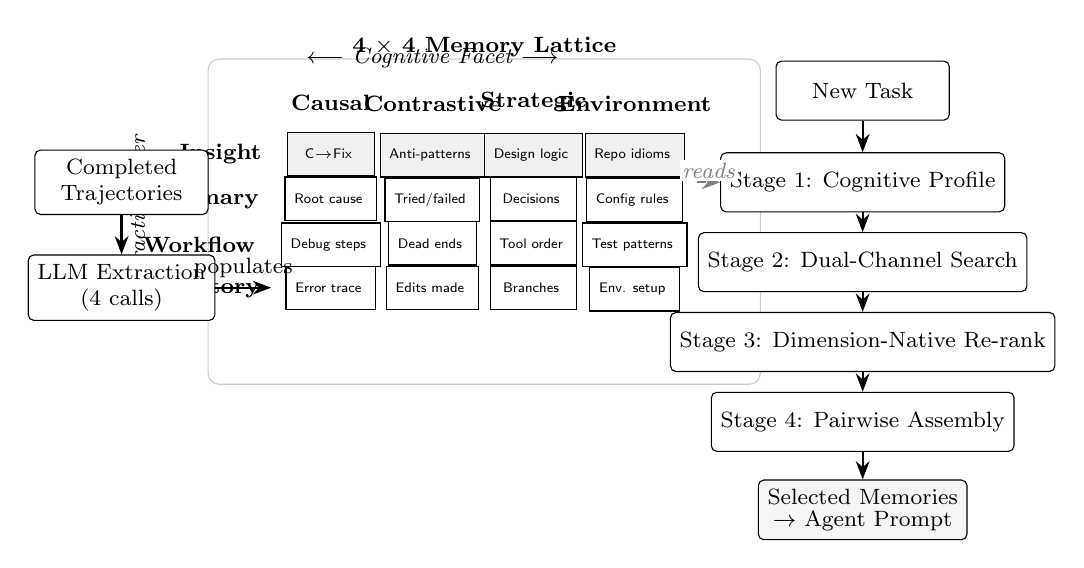
\begin{tikzpicture}[
    >=Stealth,
    box/.style={draw, rectangle, rounded corners=2pt, minimum width=22mm, minimum height=7.5mm, align=center, font=\footnotesize, fill=white},
    pipeline/.style={draw, rectangle, rounded corners=2pt, minimum width=26mm, minimum height=7.5mm, align=center, font=\footnotesize, fill=white},
    cell/.style={draw, rectangle, minimum width=11mm, minimum height=5.5mm, align=center, font=\tiny\sffamily, fill=white},
    hdr/.style={cell, fill=gray!12},
    arr/.style={->, >=Stealth, thick},
]

% === CENTER: 4x4 Cognitive Lattice ===
\matrix (L) [matrix of nodes,
    nodes={cell},
    row sep=-\pgflinewidth,
    column sep=-\pgflinewidth,
    row 1/.style={nodes={hdr}},
] {
C$\rightarrow$Fix & Anti-patterns & Design logic & Repo idioms \\
Root cause     & Tried/failed  & Decisions    & Config rules \\
Debug steps    & Dead ends     & Tool order   & Test patterns \\
Error trace    & Edits made    & Branches     & Env. setup \\
};

% --- Column labels (Cognitive Facets) ---
\node[font=\footnotesize, above=1.5mm of L-1-1] {\textbf{Causal}};
\node[font=\footnotesize, above=1.5mm of L-1-2] {\textbf{Contrastive}};
\node[font=\footnotesize, above=1.5mm of L-1-3] {\textbf{Strategic}};
\node[font=\footnotesize, above=1.5mm of L-1-4] {\textbf{Environment}};

% --- Row labels (Abstraction Tiers) ---
\node[font=\footnotesize, left=2mm of L-1-1, anchor=east] {\textbf{Insight}};
\node[font=\footnotesize, left=2mm of L-2-1, anchor=east] {\textbf{Summary}};
\node[font=\footnotesize, left=2mm of L-3-1, anchor=east] {\textbf{Workflow}};
\node[font=\footnotesize, left=2mm of L-4-1, anchor=east] {\textbf{Trajectory}};

% --- Axis labels ---
\node[font=\footnotesize\itshape, above=7mm of L-1-2] {$\longleftarrow$ Cognitive Facet $\longrightarrow$};
\node[font=\footnotesize\itshape, rotate=90] at ($(L.west) + (-17mm, 0)$) {Abstraction Tier};

% --- Background box for lattice ---
\begin{scope}[on background layer]
\node[draw=gray!40, rounded corners=4pt, inner sep=8mm, fit=(L),
      label={[font=\footnotesize\bfseries, yshift=-1mm]north:4 $\times$ 4 Memory Lattice}] {};
\end{scope}

% === LEFT: Memory Construction ===
\node[box] (traj) at ($(L.west) + (-19mm, 5mm)$) {Completed\\Trajectories};
\node[box, below=5mm of traj] (extract) {LLM Extraction\\(4 calls)};
\draw[arr] (traj) -- (extract);
\draw[arr] (extract.east) -- (extract.east -| L.west) node[midway, above, font=\footnotesize] {populates};

% === RIGHT: Retrieval Pipeline ===
\node[pipeline] (s1) at ($(L.east) + (21mm, 5mm)$) {Stage 1: Cognitive Profile};
\node[box, above=4mm of s1] (query) {New Task};
\node[pipeline, below=2.5mm of s1] (s2) {Stage 2: Dual-Channel Search};
\node[pipeline, below=2.5mm of s2] (s3) {Stage 3: Dimension-Native Re-rank};
\node[pipeline, below=2.5mm of s3] (s4) {Stage 4: Pairwise Assembly};
\node[box, below=3.5mm of s4, fill=gray!8] (result) {Selected Memories\\[-0.5ex] $\rightarrow$ Agent Prompt};

\draw[arr] (query) -- (s1);
\draw[arr] (s1) -- (s2);
\draw[arr] (s2) -- (s3);
\draw[arr] (s3) -- (s4);
\draw[arr] (s4) -- (result);

% --- Lattice → Retrieval connection ---
\draw[arr, dashed, gray] (L.east |- s1.west) -- (s1.west)
    node[midway, above, font=\footnotesize\itshape, fill=white, inner sep=1pt] {reads};

\end{tikzpicture}
\caption{System overview of \textsc{COGENT}. The 4$\times$4 memory lattice (center) organizes agent experiences along two axes: abstraction tier (vertical) and cognitive facet (horizontal). Completed trajectories are extracted into lattice entries (left). At inference time, a new task triggers cognitive profile elicitation (Stage~1), dual-channel semantic search (Stage~2), dimension-native re-ranking (Stage~3), and pairwise interaction-aware assembly (Stage~4). The selected complementary memories are injected into the agent's system prompt.}
\label{fig:architecture}
\end{figure*}

\subsubsection{Stage 1: Cognitive Profile Elicitation}

An LLM analyzes the task description and produces a cognitive profile---an assessment of how strongly each of the four cognitive facets is likely relevant to the task---alongside a causal signature hypothesizing the bug's likely anatomy. The profile text is used for the cognition-level similarity channel in Stage~2, and it gates the re-ranking in Stage~3 by identifying facets of marginal relevance whose candidates should be penalized.

\subsubsection{Stage 2: Dual-Channel Semantic Retrieval}

Two similarity channels estimate relevance for each memory. The first matches the raw task description against the repository-oriented representation of each memory, capturing concrete vocabulary overlap. The second matches the cognitive profile text against the abstract-oriented representation, capturing structural reasoning similarity independent of surface vocabulary. The two channels are fused with a weight favoring the task-level channel, so that concrete relevance anchors the retrieval while the cognitive channel recovers structurally analogous but lexically distant candidates. The top candidates by fused similarity advance to re-ranking.

\subsubsection{Stage 3: Dimension-Native Re-ranking}

Rather than assigning a single generic relevance score, each candidate is evaluated by the criterion \emph{native to its own cognitive facet}: Causal entries by structural alignment between stored and hypothesized causal chains; Contrastive entries by whether their anti-pattern or success pattern bears on the query's likely failure mode; Strategic entries by the portability of their methodological guidance; and Environment entries by the overlap between described and implicated repository regions. For facets the cognitive profile flags as low-need, dimension scores receive a penalty---a highly scored causal memory is unhelpful when the query primarily needs operational knowledge.

The candidates' cognitive abstracts are bundled into a single batch LLM call. The final score fuses semantic similarity from Stage~2 with the dimension-native score, with cognitive structure fit receiving the larger weight.

\subsubsection{Stage 4: Pairwise Interaction-Aware Assembly}

A greedy procedure constructs the output set round by round, starting from the highest-scoring candidate. In each subsequent round, remaining candidates are re-evaluated against already-chosen memories through two lenses: a \textbf{redundancy} penalty when a candidate shares both the abstraction tier and cognitive facet of an already-selected memory and the two are highly similar, and a \textbf{complementarity} bonus when a candidate originates from the same source task but belongs to a different cognitive facet (enhanced for Causal--Environment dyads). The candidate with the highest adjusted score is added to the set.

After assembly, we apply a batch-adaptive quality filter. A score threshold $\tau$ is computed from the distribution of the full $N=20$ candidate pool (not just the selected $K$)---using the full pool yields reliable statistics, which $K=3$ samples would not provide---as $\tau = \max(\tau_{\text{floor}},\; \text{median}(\{\text{combined}_i\}) - \lambda \cdot \sigma(\{\text{combined}_i\}))$, with $\tau_{\text{floor}} = 0.45$ and $\lambda = 0.5$. This threshold is then applied to the selected memories: any whose combined score falls below $\tau$ are discarded, with a minimum of one memory always retained. The threshold tightens when the candidate batch is uniformly high-quality (encouraging selectivity) and relaxes to the floor when scores are diffuse (preventing all memories from being discarded in a low-quality batch).

The pairwise adjustments are rule-based rather than learned \cite{context-picker, memfly}, requiring no training data and remaining fully interpretable.

% ----------------------------------------------------------------------
\subsection{Sequential Memory Accumulation}
\label{sec:pool}

\textsc{COGENT} operates under a sequential accumulation protocol. Tasks are processed in a fixed order and the memory pool expands after each episode: a task is solved using memories from all previously processed tasks, its trajectory is then extracted into lattice entries, and these entries become immediately available for all subsequent tasks. A batch regime---where a fixed set of source tasks populates a static pool---is also supported for offline evaluation, though the sequential mode is the primary protocol in this work.

This design mirrors continual deployment: the agent accumulates experience over time, and each episode benefits from the full history of prior resolutions. Beyond its practical motivation, the sequential regime enables direct measurement of each task's \emph{marginal contribution} to downstream performance. By tracking cumulative pass rates as the pool grows, one can observe how incremental memory value evolves and at what point saturation begins.

% ======================================================================
\section{Experimental Design}

All experiments described below have been implemented and are currently executing. We report the complete experimental design; the full system (E1) and no-memory baseline (E6) results are from completed runs, while cell values for E2--E5 and E7--E17, E25--E26 are marked as pending where runs have not yet finished.\footnote{Code and configuration files for reproducing all experiments are available in the project repository under \texttt{harbor/configs/experiments/}.}

\subsection{Setup}

\textbf{Corpus.} 100 overlapping tasks sampled (seed 42) from the SWE-bench Verified Django subset \cite{swe-bench}. Each task pairs a natural-language issue description with a held-out test suite for mechanical verification.

\textbf{Agent and Model.} mini-swe-agent as the base agent, DeepSeek-V4-Flash as the backend LLM (\texttt{deepseek-chat}, temperature 0). Embeddings via SentenceTransformer's all-MiniLM-L6-v2 (384-dimensional). All experiments share identical model configuration; the agent is allotted a maximum of 150 steps per task. The no-memory baseline uses a standard system prompt containing only agent instructions and the task description.

\textbf{Evaluation.} Primary metric: pass@1 (single attempt per task). Secondary: counts of baseline-failure$\rightarrow$COGENT-success (improvements) and baseline-success$\rightarrow$COGENT-failure (regressions). Sequential experiments additionally track cumulative pass rate as a function of pool size.

\textbf{Full System Configuration (E1).} $\alpha_{\text{dual}} = 0.70$, $N = 20$, $\alpha_s = 0.35$, $\alpha_c = 0.65$, $K = 3$, $\tau_{\text{floor}} = 0.45$, $\lambda = 0.5$, redundancy cosine threshold $0.92$. All experiments use the sequential execution protocol with identical task ordering (random seed 42) for cross-experiment comparability.

\subsection{Core Pipeline Ablation Ladder (E1--E6)}

Table~\ref{tab:ablation-config} defines a six-experiment ablation ladder that progressively strips components from the full system, answering a sequence of nested questions about each component's marginal value.

\begin{table}[t]
\centering
\caption{Configuration matrix for E1--E6. All share: sequential regime, 100 tasks (seed 42), mini-swe-agent, DeepSeek-V4-Flash, step limit 150.}
\label{tab:ablation-config}
\begin{tabular}{lccccc}
\toprule
\textbf{ID} & \textbf{Memory Structure} & \textbf{Rerank} & \textbf{Synergy} & \textbf{Channels} & \textbf{Threshold} \\
\midrule
E1 (Full)   & $4{\times}4$ cognitive lattice & \checkmark & \checkmark & Dual   & Adaptive \\
E2          & $4{\times}4$ cognitive lattice & ---        & \checkmark & Dual   & Adaptive \\
E3          & $4{\times}4$ cognitive lattice & \checkmark & ---        & Dual   & Adaptive \\
E4          & $4{\times}4$ cognitive lattice & ---        & ---        & Single & Fixed   \\
E5          & MTL three-tier (flat)         & ---        & ---        & Single & Fixed   \\
E6          & None (baseline)               & ---        & ---        & ---    & ---     \\
\bottomrule
\end{tabular}
\end{table}

The ladder addresses five nested comparisons:

\begin{itemize}
    \item \textbf{E5 vs.\ E6}: Does \emph{any} memory---even without cognitive facet structure---improve over the no-memory baseline? Quantifies the value of memory per se.
    \item \textbf{E4 vs.\ E5}: What is the incremental gain from replacing a flat three-tier scheme with the $4 \times 4$ cognitive lattice, while holding the retrieval mechanism constant (pure embedding, no LLM augmentation)? Isolates the representational contribution of the two-axis cognitive organization.
    \item \textbf{E2 vs.\ E1}: How much does dimension-native LLM re-ranking (Stage 3) contribute beyond dual-channel embedding alone? Isolates the value of facet-native scoring criteria.
    \item \textbf{E3 vs.\ E1}: What is the independent contribution of pairwise interaction-aware assembly (Stage 4)? Isolates the value of explicit redundancy/complementarity modeling within the selected set.
    \item \textbf{E4 vs.\ E1}: Spanning the full range from pure embedding to the complete pipeline, what is the total gain attributable to the LLM-based cognitive components (re-ranking + interaction-aware selection) jointly?
\end{itemize}

\subsection{Cognitive Facet Leave-One-Out (E7--E10)}

To verify that each cognitive facet contributes non-redundant information, we ablate one facet at a time from the full $4 \times 4$ lattice, retaining the complete LLM pipeline:

\begin{itemize}
    \item \textbf{E7 (--Causal)}: Pool restricted to Contrastive + Strategic + Environment across all tiers.
    \item \textbf{E8 (--Contrastive)}: Pool restricted to Causal + Strategic + Environment.
    \item \textbf{E9 (--Strategic)}: Pool restricted to Causal + Contrastive + Environment.
    \item \textbf{E10 (--Environment)}: Pool restricted to Causal + Contrastive + Strategic.
\end{itemize}

A significant pass-rate drop when a facet is removed constitutes evidence that the facet encodes information the remaining three cannot compensate for. A negligible drop suggests redundancy or coverage by remaining facets.

\subsection{Abstraction Tier Leave-One-Out (E11--E13)}

A parallel analysis ablates the abstraction axis, removing one tier across all four facets:

\begin{itemize}
    \item \textbf{E11 (--Trajectory)}: Pool restricted to Workflow + Summary.
    \item \textbf{E12 (--Workflow)}: Pool restricted to Trajectory + Summary.
    \item \textbf{E13 (--Summary)}: Pool restricted to Trajectory + Workflow.
\end{itemize}

Tests whether fine-grained command detail, procedural structure, and diagnostic synthesis each independently contribute to retrieval quality.

\subsection{Retrieval Robustness Checks (E14--E17)}

Four experiments probe specific design choices:

\begin{itemize}
    \item \textbf{E14 (Random Memory)}: Replace the entire retrieval pipeline with uniform random sampling of $K=3$ memories. Establishes a lower bound on retrieval quality.
    \item \textbf{E15 (LLM Direct Top-K)}: Bypass the cognitive facet taxonomy---present all $N=20$ candidates (without facet labels) to the LLM and ask it to directly select the best $K=3$. Tests whether explicit facet structure adds value beyond implicit LLM judgment.
    \item \textbf{E16 (Fixed Threshold)}: Disable adaptive thresholding ($\lambda = 0$), using a constant cutoff $\tau = 0.45$. Isolates whether distribution-aware thresholding provides measurable benefit.
    \item \textbf{E17 (No Insight Attachment)}: Suppress the mechanism linking abstract Insight-tier memories to their sibling concrete memories. Measures the value of decontextualized methodological principles alongside specific operational knowledge.
\end{itemize}

\subsection{Multi-Model Validation (E25--E26)}

To assess model-agnostic generalizability, the full system (E1 configuration) is replicated with GPT-4o (E25) and Claude Opus 4.5 (E26) as the backbone model.

\subsection{Main Results (Completed)}

\begin{table}[t]
\centering
\caption{Main results on SWE-bench Verified Django subset (100 tasks).}
\label{tab:main-results}
\begin{tabular}{lccc}
\toprule
\textbf{Condition} & \textbf{Pass Rate} & \textbf{Improved} & \textbf{Regressed} \\
\midrule
No Memory (Baseline, E6) & 56.0\% & --- & --- \\
\textsc{COGENT} (Full, E1)  & \textbf{76.0\%} & 22 & 2 \\
\bottomrule
\end{tabular}
\end{table}

Table~\ref{tab:main-results} presents the headline comparison. The 20 percentage point net gain decomposes into 22 tasks newly solved and 2 regressed. Improvements span recurring defect categories: database migration ordering violations (7), template rendering logic errors (5), URL dispatch and middleware misconfiguration (4), form validation edge cases (3), and serialization inconsistencies (3). Gains concentrate in two categories: (i) tasks whose causal structure has strong precedent in the memory pool (e.g., migration dependency violations, which exhibit highly stereotyped error$\to$cause$\to$fix chains), and (ii) environment-knowledge-intensive tasks where the agent otherwise spends many steps re-discovering operational details (e.g., test invocation idioms, fixture loading behavior).

\subsection{Ablation Results (Pending)}
\label{sec:ablation-pending}

\begin{table}[t]
\centering
\caption{Ablation result structure. ``TBD'' cells correspond to experiments currently executing.}
\label{tab:ablation-results}
\begin{tabular}{lcc}
\toprule
\textbf{Condition} & \textbf{Pass Rate} & \textbf{$\Delta$ from E1} \\
\midrule
E1: Full \textsc{COGENT} & 76.0\% & --- \\
E2: No Dimension-Native Rerank & TBD & TBD \\
E3: No Pairwise Interaction Assembly & TBD & TBD \\
E4: Pure Embedding (no LLM stages) & TBD & TBD \\
E5: MTL Three-Tier (no facets) & TBD & TBD \\
E6: No Memory & 56.0\% & $-20.0$ pp \\
\midrule
\multicolumn{3}{c}{\textit{Facet Leave-One-Out}} \\
\midrule
E7: --Causal & TBD & TBD \\
E8: --Contrastive & TBD & TBD \\
E9: --Strategic & TBD & TBD \\
E10: --Environment & TBD & TBD \\
\midrule
\multicolumn{3}{c}{\textit{Tier Leave-One-Out}} \\
\midrule
E11: --Trajectory & TBD & TBD \\
E12: --Workflow & TBD & TBD \\
E13: --Summary & TBD & TBD \\
\midrule
\multicolumn{3}{c}{\textit{Robustness Checks}} \\
\midrule
E14: Random Memory & TBD & TBD \\
E15: LLM Direct Top-K (no facets) & TBD & TBD \\
E16: Fixed Threshold & TBD & TBD \\
E17: No Insight Attachment & TBD & TBD \\
\midrule
\multicolumn{3}{c}{\textit{Multi-Model}} \\
\midrule
E25: GPT-4o (Full Pipeline) & TBD & TBD \\
E26: Claude Opus 4.5 (Full Pipeline) & TBD & TBD \\
\bottomrule
\end{tabular}
\end{table}

\subsection{Regression Case Analysis}

Two tasks deteriorated when memory was introduced. We analyze each to understand failure modes.

\textbf{\texttt{django-13807}.} The core issue is an interaction between Django's \texttt{refresh\_from\_db()} and a user-defined \texttt{@property} that shadows a database column. Retrieved causal memories concerning model field access patterns scored highly, but pertained to \emph{deferred attribute loading}---a mechanism structurally adjacent yet causally distinct from property-based field shadowing. The agent, guided by the retrieved memory, probed the deferred loading infrastructure before recognizing the actual mechanism. This exposes a limitation of causal-structure matching: when two phenomena share a similar surface causal signature (``accessing a model attribute returns unexpected data'') but differ in underlying mechanism, even dimension-native scoring can produce false positives. A finer-grained \emph{mechanism-level} distinction within the Causal facet could mitigate this error class.

\textbf{\texttt{django-14053}.} A namespace collision in Django's admin template tag registration requiring a three-line local edit. Retrieved strategic memories about ``encapsulating template rendering logic'' and a contrastive anti-pattern warning against ``global template state mutation'' steered the agent toward an unnecessarily broad restructuring. This illustrates a failure mode of strategic-tier memory: abstract methodological principles can bias toward over-engineered solutions when the true fix is narrow and context-specific.

\subsection{Planned Analyses}

Upon completion of the ablation suite, we will conduct the following:

\textbf{Cumulative pass rate vs.\ pool size.} Plotting the pass rate over rounds $1 \ldots t$ against the accumulating pool size reveals marginal memory value. We anticipate three regimes: rapid early improvement (pool sizes 1--15, each new task adding substantial novel cognitive coverage), decelerating gains (16--50, filling increasingly specific cognitive niches), and near-saturation (beyond $\sim$50, additional entries largely recapitulating represented patterns). This trajectory would parallel cognitive load saturation documented in human memory research \cite{cognitive-load}, wherein retrieval interference eventually offsets the benefit of additional stored information \cite{ctim-rover}.

\textbf{Facet selection frequency.} Aggregating cognitive facet labels of all top-$K$ retrieved memories across all tasks will characterize which reasoning assistance types the system empirically favors. Preliminary inspection suggests Causal dominates (diagnostic reasoning as the central debugging activity), followed by Environment (operational knowledge), Strategic (methodology), and Contrastive (anti-pattern recognition, likely valuable selectively when the agent explores wrong directions).

% ======================================================================
\section{Conclusion}

We presented \textsc{COGENT}, a memory framework for LLM-based code agents organized around a cognitive facet taxonomy---Causal, Contrastive, Strategic, and Environment---crossed with abstraction tiers to produce a $4 \times 4$ memory lattice. The retrieval pipeline elicits a cognitive profile from incoming queries, conducts dual-channel embedding search (task-level and cognition-level), performs dimension-native re-ranking where each memory is scored by its own facet's criteria, and assembles a complementary memory set with pairwise interaction adjustments. The framework operates entirely through prompt injection with zero model training.

\textbf{Limitations.} (1) Memory construction incurs a fixed 5 LLM calls per completed task; amortizing extraction across batches of structurally similar tasks could reduce cost at scale. (2) The cognitive facet taxonomy is specified a priori; whether data-driven facet discovery from agent trajectories would yield a more effective partition remains open. (3) Current evaluation is scoped to a single repository ecosystem (Django) and agent framework (mini-swe-agent); cross-repository and cross-agent generalization require dedicated study. (4) Regression cases reveal that high-scoring cognitive matches can misdirect the agent when surface causal similarity masks underlying mechanistic divergence, motivating finer-grained discrimination within the Causal facet.

\textbf{Future Work.} Key directions include: (1) empirically refining the facet inventory through systematic analysis of failure modes across diverse repositories and languages; (2) building mechanism-level causal discriminators to suppress false-positive retrievals; (3) investigating learned, repository-adaptive facet weights; (4) broadening evaluation to AIME, LiveCodeBench, and USACO; and (5) exploring cross-agent knowledge transfer where memories harvested by one agent architecture benefit a different implementation.

% ======================================================================
\section*{Acknowledgments}

% TODO

% ======================================================================
\begin{thebibliography}{}

\bibitem[Lewis et al., 2020]{rag-lewis}
Lewis, P.; Perez, E.; Piktus, A.; Petroni, F.; Karpukhin, V.; Goyal, N.; K\"{u}ttler, H.; Lewis, M.; Yih, W.; Rockt\"{a}schel, T.; Riedel, S.; and Kiela, D.
\newblock Retrieval-augmented generation for knowledge-intensive {NLP} tasks.
\newblock In \emph{NeurIPS}, 2020.

\bibitem[Yang et al., 2024]{swe-agent}
Yang, J.; Jimenez, C. E.; Wettig, A.; Lieret, K.; Yao, S.; Narasimhan, K.; and Press, O.
\newblock {SWE}-Agent: Agent-computer interfaces enable automated software engineering.
\newblock In \emph{NeurIPS}, 2024.

\bibitem[mini-swe-agent]{mini-swe-agent}
mini-swe-agent: A lightweight software engineering agent.
\newblock \emph{https://github.com/ethanmooney/mini-swe-agent}, 2024.

\bibitem[Wang et al., 2024]{openhands}
Wang, X.; et al.
\newblock {OpenHands}: An open platform for {AI} software developers as generalist agents.
\newblock \emph{arXiv preprint arXiv:2407.16741}, 2024.

\bibitem[Zhang et al., 2024]{autocoderover}
Zhang, Y.; et al.
\newblock {AutoCodeRover}: Autonomous program improvement.
\newblock In \emph{Proceedings of ISSTA}, 2024.

\bibitem[Shinn et al., 2023]{reflexion}
Shinn, N.; Cassano, F.; Gopinath, A.; Narasimhan, K.; and Yao, S.
\newblock {Reflexion}: Language agents with verbal reinforcement learning.
\newblock In \emph{NeurIPS}, 2023.

\bibitem[Zhao et al., 2024]{expel}
Zhao, A.; Huang, D.; Xu, Q.; Lin, M.; Liu, Y.-J.; and Huang, G.
\newblock {ExpeL}: {LLM} agents are experiential learners.
\newblock In \emph{Proceedings of AAAI}, 2024.

\bibitem[Lindenbauer et al., 2025]{ctim-rover}
Lindenbauer, M.; et al.
\newblock From knowledge to noise: {CTIM}-Rover and the pitfalls of episodic memory in software engineering agents.
\newblock In \emph{Proceedings of REALM (ACL Workshop)}, 2025.

\bibitem[Lingam et al., 2024]{dot-bank}
Lingam, V.; et al.
\newblock {DoT-Bank}: Diverse self-reflections and exemplar trajectories for agent memory.
\newblock \emph{arXiv preprint}, 2024.

\bibitem[agent-workflow-memory]{awm}
Agent Workflow Memory.
\newblock \emph{arXiv preprint}, 2024.

\bibitem[Packer et al., 2023]{memgpt}
Packer, C.; Fang, V.; Patil, S. G.; Lin, K.; Wooders, S.; and Gonzalez, J. E.
\newblock {MemGPT}: Towards {LLMs} as operating systems.
\newblock \emph{arXiv preprint arXiv:2310.08560}, 2023.

\bibitem[Park et al., 2023]{generative-agents}
Park, J. S.; O'Brien, J. C.; Cai, C. J.; Morris, M. R.; Liang, P.; and Bernstein, M. S.
\newblock Generative agents: Interactive simulacra of human behavior.
\newblock In \emph{Proceedings of UIST}, 2023.

\bibitem[Zhang et al., 2025]{g-memory}
Zhang, Y.; et al.
\newblock {G-Memory}: Tracing hierarchical memory for multi-agent systems.
\newblock In \emph{NeurIPS}, 2025.

\bibitem[Shah et al., 2025]{evolve-mem}
Shah, R.; et al.
\newblock {EVOLVE-MEM}: A self-adaptive hierarchical memory architecture for next-generation agentic {AI} systems.
\newblock In \emph{NeurIPS}, 2025.

\bibitem[h-mem]{h-mem}
{H-MEM}: Hierarchical memory for high-efficiency long-term reasoning.
\newblock \emph{arXiv preprint arXiv:2507.22925}, 2025.

\bibitem[context-picker]{context-picker}
{Context-Picker}: Reasoning-aware variable-length evidence selection under a token budget.
\newblock \emph{arXiv preprint arXiv:2512.14465}, 2025.

\bibitem[mem1]{mem1}
{MEM1}: Learning to synergize memory and reasoning for efficient long-horizon agents.
\newblock In \emph{NeurIPS}, 2025.

\bibitem[memfly]{memfly}
{MemFly}: On-the-fly memory optimization via information bottleneck.
\newblock \emph{arXiv preprint arXiv:2602.07885}, 2025.

\bibitem[dcpm]{dcpm}
Memory beyond recall: A dual-process cognitive memory system for self-evolving {LLM} agents.
\newblock \emph{arXiv preprint arXiv:2606.09483}, 2025.

\bibitem[cdmem]{cdmem}
Context-dependent memory for {LLM} agents.
\newblock In \emph{Proceedings of NAACL (Industry Track)}, 2025.

\bibitem[Tulving, 1972]{tulving-episodic}
Tulving, E.
\newblock Episodic and semantic memory.
\newblock In \emph{Organization of Memory}, Academic Press, 1972.

\bibitem[Tulving and Thomson, 1973]{tulving-encoding}
Tulving, E.; and Thomson, D. M.
\newblock Encoding specificity and retrieval processes in episodic memory.
\newblock \emph{Psychological Review}, 80(5):352--373, 1973.

\bibitem[Schank, 1982]{schank-dynamic}
Schank, R. C.
\newblock \emph{Dynamic Memory: A Theory of Reminding and Learning in Computers and People}.
\newblock Cambridge University Press, 1982.

\bibitem[Sweller, 1988]{cognitive-load}
Sweller, J.
\newblock Cognitive load during problem solving: Effects on learning.
\newblock \emph{Cognitive Science}, 12(2):257--285, 1988.

\bibitem[Reimers and Gurevych, 2019]{sentence-transformers}
Reimers, N.; and Gurevych, I.
\newblock {Sentence-BERT}: Sentence embeddings using {Siamese} {BERT}-networks.
\newblock In \emph{Proceedings of EMNLP-IJCNLP}, 2019.

\bibitem[Jimenez et al., 2024]{swe-bench}
Jimenez, C. E.; Yang, J.; Wettig, A.; Yao, S.; Pei, K.; Press, O.; and Narasimhan, K.
\newblock {SWE}-bench: Can language models resolve real-world {GitHub} issues?
\newblock In \emph{ICLR}, 2024.

\bibitem[Feng et al., 2020]{codebert}
Feng, Z.; Guo, D.; Tang, D.; Duan, N.; Feng, X.; Gong, M.; Shou, L.; Qin, B.; Liu, T.; Jiang, D.; and Zhou, M.
\newblock {CodeBERT}: A pre-trained model for programming and natural languages.
\newblock In \emph{Findings of EMNLP}, 2020.

\bibitem[Wang et al., 2021]{codet5}
Wang, Y.; Wang, W.; Joty, S.; and Hoi, S. C.
\newblock {CodeT5}: Identifier-aware unified pre-trained encoder-decoder models for code understanding and generation.
\newblock In \emph{Proceedings of EMNLP}, 2021.

\bibitem[Roziere et al., 2023]{code-llama}
Rozi\`{e}re, B.; et al.
\newblock {Code Llama}: Open foundation models for code.
\newblock \emph{arXiv preprint arXiv:2308.12950}, 2023.

\bibitem[Brown et al., 2020]{icl}
Brown, T.; et al.
\newblock Language models are few-shot learners.
\newblock In \emph{NeurIPS}, 2020.

\bibitem[ActMem, 2025]{actmem}
{ActMem}: Bridging the gap between memory retrieval and reasoning in {LLM} agents.
\newblock \emph{arXiv preprint arXiv:2603.00026}, 2025.

\end{thebibliography}

\end{document}
